%! Author = Juniell
%! Date = 10.05.2021

% Preamble
\documentclass[a4paper, 14pt]{extarticle}

% Packages
\usepackage[T2A]{fontenc}
\usepackage{natbib}
\usepackage{graphicx}
\usepackage[english, russian]{babel}
\usepackage{fontspec}
\usepackage{amsmath}
\usepackage{amsfonts}
\usepackage{amssymb}
\usepackage{amsthm}
\usepackage{mathtools}
\usepackage{mathrsfs}
\usepackage{fullpage}
\usepackage{ulem}
\usepackage{setspace}
\usepackage{listings}
\usepackage{indentfirst}
\usepackage[left=2cm,right=1.5cm,top=2cm,bottom=2cm]{geometry}
\usepackage{xcolor}
\usepackage{float}
\usepackage{csquotes}
\usepackage{hyperref}
\usepackage{graphics}

\definecolor{urlcolor}{HTML}{0000FF} % цвет ссылок
\definecolor{linkcolor}{HTML}{000000} % цвет гиперссылок
\hypersetup{pdfstartview=FitH, linkcolor=linkcolor, urlcolor=urlcolor, colorlinks=true}

\setmainfont{Times New Roman}
\setlength{\parindent}{5ex}
\setlength{\parskip}{1em}
\renewcommand{\baselinestretch}{1}

\graphicspath{{resources/Images}}

\definecolor{buzzlightyear}{HTML}{8757A5}
\definecolor{grass}{HTML}{738D06}
\definecolor{literal}{HTML}{F18A2B}
\definecolor{commentcolor}{HTML}{8E908B}

\lstdefinestyle{habrstyle}{
    backgroundcolor=\color{white},
    commentstyle=\color{commentcolor},
    keywordstyle=\bfseries\color{buzzlightyear},
    numberstyle=\tiny\color{commentcolor},
    stringstyle=\color{grass},
    basicstyle=\ttfamily\footnotesize,
    breakatwhitespace=false,
    breaklines=true,
    captionpos=b,
    keepspaces=true,
    numbers=left,
    numbersep=5pt,
    showspaces=false,
    showstringspaces=false,
    showtabs=false,
    tabsize=4,
    language=Python
}

\lstset{style=habrstyle}


% Document
\begin{document}
% Титульный лист
    \begin{center}
        \begin{center}
            \hfill \break
            \normalsize{Санкт-Петербургский государственный политехнический}\\
            \normalsize{университет Петра Великого}\\
            \hfill \break
            \normalsize{\textbf{Высшая школа интеллектуальных систем и}}\\
            \normalsize{\textbf{суперкомпьютерных технологий}}\\
            \hfill \break
            \hfill \break
            \hfill \break
            \hfill \break
            \hfill \break
            \normalsize{Отчёт по лабораторной работе №8}\\
            \normalsize{Дисциплина: Телекоммуникационные технологии}\\
            \normalsize{Тема: Фильтрация и свёртка}\\
        \end{center}
        \hfill \break
        \hfill \break
        \hfill \break
        \hfill \break
        \hfill \break
        \hfill \break
        \hfill \break
        \hfill \break
        \hfill \break
        \hfill \break
        \begin{tabbing}
            Выполнил студент гр. 3530901/80201 \`В.А. Пучкина\\
            \\
            Преподаватель: \`Н.В. Богач\\
        \end{tabbing}
        \hfill \break
        \hfill \break
        \hfill \break
        \hfill \break
        \begin{center}
            Санкт-Петербург\\
            2021
        \end{center}
        \thispagestyle{empty}
    \end{center}

% Оглавление
    \newpage
    \tableofcontents

% Список иллюстраций
    \newpage
    \listoffigures

% Список листингов
    \newpage
    \lstlistoflistings

% ---------------------------------------------- Упражнение 8.1 ----------------------------------------------
    \newpage
    \section{Упражнение 8.1}
    \label{sec:task1}

    В этом упражнении необходимо изучить примеры в файле \texttt{chap08.ipynb}. Также следует проверить, что будет
    происходить при увеличении ширины гауссова окна \texttt{std} без увеличения числа элементов в окне \texttt{M}.

    Итак, изучив все примеры, приступим к эксперименту.

    Установим \texttt{M} = 40 и \texttt{std} = 1.

    \begin{figure}[h]
        \centering
        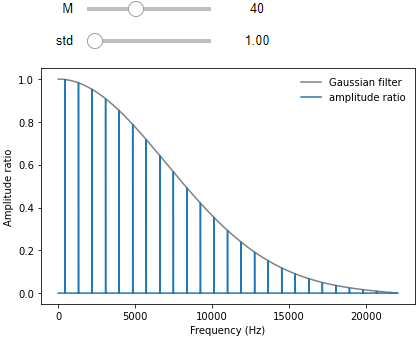
\includegraphics[width=0.8\linewidth]{resources/Images/task1_check_m40_std1}
        \caption{\texttt{M} = 40 и \texttt{std} = 1.}
        \label{fig:task1_check_m40_std1}
    \end{figure}

    Теперь установим \texttt{M} = 40 и \texttt{std} = 3.

    \begin{figure}[H]
        \centering
        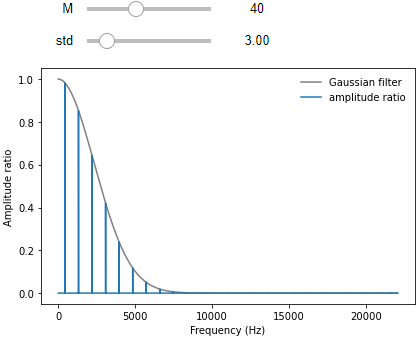
\includegraphics[width=0.75\linewidth]{resources/Images/task1_check_m40_std3}
        \caption{\texttt{M} = 40 и \texttt{std} = 3.}
        \label{fig:task1_check_m40_std3}
    \end{figure}

    Установим \texttt{M} = 40 и \texttt{std} = 5.

    \begin{figure}[h]
        \centering
        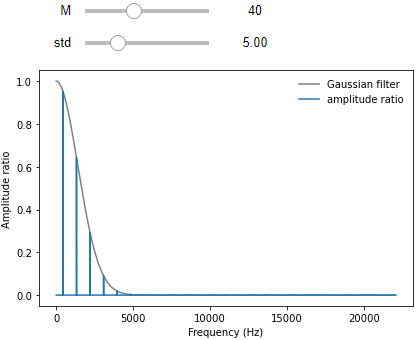
\includegraphics[width=0.75\linewidth]{resources/Images/task1_check_m40_std5}
        \caption{\texttt{M} = 40 и \texttt{std} = 5.}
        \label{fig:task1_check_m40_std5}
    \end{figure}

    И наконец, проверим при \texttt{M} = 40 и \texttt{std} = 20.

    \begin{figure}[h]
        \centering
        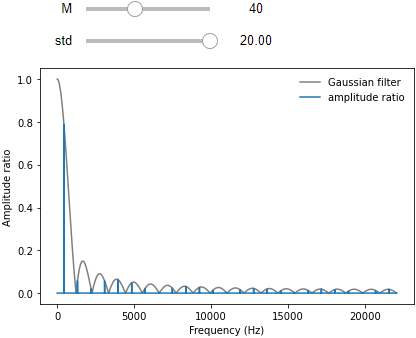
\includegraphics[width=0.8\linewidth]{resources/Images/task1_check_m40_std20}
        \caption{\texttt{M} = 40 и \texttt{std} = 20.}
        \label{fig:task1_check_m40_std20}
    \end{figure}

    Из полученных результатов можно заметить, что без увеличения \texttt{M} но при увеличении \texttt{std} окно
    резко сужается, высокочастотные гармоники в спектре падают, после чего появляются колебания, называемые
    <<боковыми лепестками>>.

    \newpage

% ---------------------------------------------- Упражнение 8.2 ----------------------------------------------
    \section{Упражнение 8.2}
    \label{sec:task2}

    В этом упражнении необходимо убедиться, что преобразование Фурье гауссовой кривой - это тоже гауссова кривая.
    Также следует проверить, что происходит с преобразованием Фурье при изменении \texttt{std}.

    Итак, начнём с преобразования Фурье гауссовой кривой. Создадим гауссову кривую.

    \begin{lstlisting}[caption= Создание гауссовой кривой., label={lst:task2_gaussian}]
gaussian = scipy.signal.gaussian(M=32, std=2)
gaussian /= sum(gaussian)
plt.plot(gaussian)
decorate(xlabel='Index')    \end{lstlisting}

    \begin{figure}[h]
        \centering
        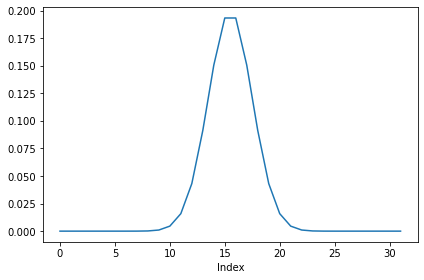
\includegraphics[width=0.8\linewidth]{resources/Images/task2_gaussian}
        \caption{Гауссово окно.}
        \label{fig:task2_gaussian}
    \end{figure}

    Теперь получим БПФ.

    \begin{lstlisting}[caption= Получение БПФ., label={lst:task2_fft}]
fft_gaussian = numpy.fft.fft(gaussian)
plt.plot(abs(fft_gaussian))
decorate(xlabel='Frequency (Hz)', ylabel='Amplitude')   \end{lstlisting}

    Осуществим сдвиг отрицательных частот.

    \begin{lstlisting}[caption= Сдвиг отрицательных частот., label={lst:task2_rolled}]
N = len(gaussian)
fft_rolled = numpy.roll(fft_gaussian, N//2)
plt.plot(abs(fft_rolled))
decorate(xlabel='Frequency (Hz)', ylabel='Amplitude')   \end{lstlisting}

    \begin{figure}[H]
        \centering
        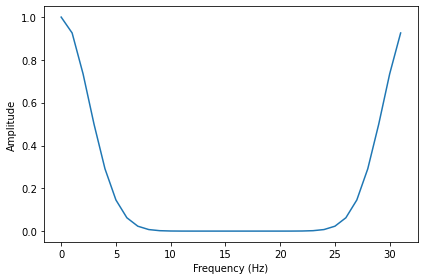
\includegraphics[width=0.8\linewidth]{resources/Images/task2_fft}
        \caption{БПФ.}
        \label{fig:task2_fft}
    \end{figure}

    \begin{figure}[H]
        \centering
        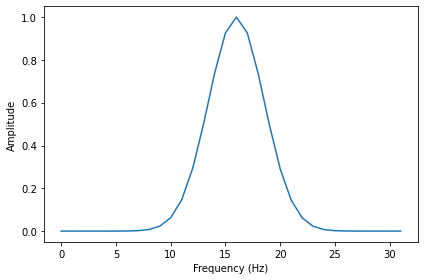
\includegraphics[width=0.8\linewidth]{resources/Images/task2_rolled}
        \caption{Сдвинутое БПФ.}
        \label{fig:task2_rolled}
    \end{figure}

    Полученный результат (Рис.\ref{fig:task2_rolled}) действительно напоминает гауссову кривую (для сравнения
    оригинальная кривая - Рис.\ref{fig:task2_gaussian}).

    Теперь перейдём к проверке влияния изменения \texttt{std} на преобразование Фурье. Для этого реализуем функцию,
    отображающую окно Гаусса и его БПФ.

    \begin{lstlisting}[caption= Функция \texttt{plot\_gaussian}., label={lst:task2_plot_gaussian}]
def plot_gaussian(std):
    M = 32
    gaussian = scipy.signal.gaussian(M=M, std=std)
    gaussian /= sum(gaussian)

    plt.subplot(1, 2, 1)
    plt.plot(gaussian)
    decorate(xlabel='Time')

    fft_gaussian = numpy.fft.fft(gaussian)
    fft_rolled = numpy.roll(fft_gaussian, M//2)

    plt.subplot(1, 2, 2)
    plt.plot(numpy.abs(fft_rolled))
    decorate(xlabel='Frequency')
    plt.show()  \end{lstlisting}

    Теперь добавим слайдер, с помощью которого будет удобно наблюдать за результатом изменения \texttt{std}.

    \begin{lstlisting}[caption= Добавление слайдера., label={lst:task2_slider}]
slider = widgets.FloatSlider(min=0.1, max=10, value=2)
interact(plot_gaussian, std=slider);    \end{lstlisting}

    И теперь проверим, как будет влиять изменение \texttt{std}. Сначала установим \texttt{std} = 2.

    \begin{figure}[H]
        \centering
        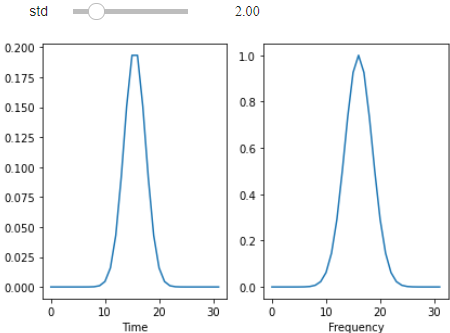
\includegraphics[width=0.75\linewidth]{resources/Images/task2_std2}
        \caption{Гауссово окно и его БПФ (\texttt{std} = 2).}
        \label{fig:task2_std2}
    \end{figure}

    \begin{figure}[H]
        \centering
        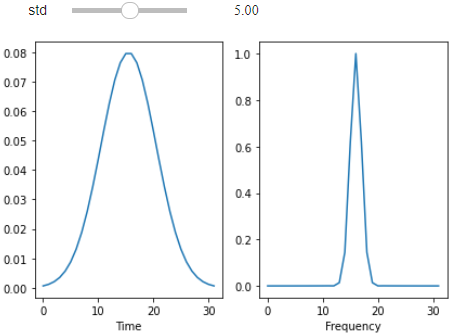
\includegraphics[width=0.8\linewidth]{resources/Images/task2_std5}
        \caption{Гауссово окно и его БПФ (\texttt{std} = 5).}
        \label{fig:task2_std5}
    \end{figure}

    \begin{figure}[H]
        \centering
        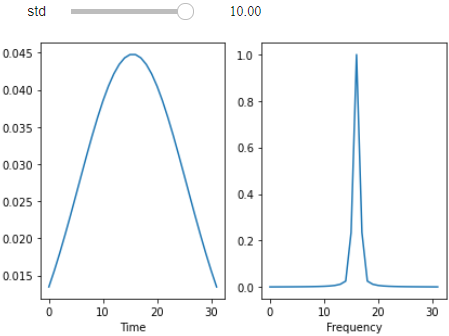
\includegraphics[width=0.8\linewidth]{resources/Images/task2_std10}
        \caption{Гауссово окно и его БПФ (\texttt{std} = 10).}
        \label{fig:task2_std10}
    \end{figure}

    Таким образом, можно заметить, что при увеличении \texttt{std} гауссово окно сжимается, а его БПФ расширяется.

    В данном упражнении была проведена работа по получению преобразования Фурье гауссовой кривой. Было доказано, что
    преобразование Фурье гауссовой кривой - это тоже гауссова кривая. Затем была проведена проверка влияния изменения
    \texttt{std} на преобразование Фурье. Был сделан вывод, при увеличении \texttt{std} гауссово окно сжимается, а его
    БПФ расширяется. Таким образом, между ними существует обратная зависимость.

    \newpage

% ---------------------------------------------- Упражнение 8.3 ----------------------------------------------
    \section{Упражнение 8.3}
    \label{sec:task3}

    В лабораторной работе №3 изучалось влияние спектра окна Хэмминга и некоторых других окон на утечки. Чтобы лучше
    разобраться в этом вопросе, изучим их ДПФ.

    Итак, сначала создадим прямоугольный сигнал и  получим его \texttt{wave}.

    \begin{lstlisting}[caption= Создание прямоугольного сигнала., label={lst:task3_square}]
signal = SquareSignal(freq=440)
wave = signal.make_wave(duration=1.0, framerate=44100)  \end{lstlisting}

    Теперь создадим окна и изучим их графики.

    \begin{lstlisting}[caption= Построение графиков окон., label={lst:task3_windows}]
M = 15
std = 2.5

gaussian = scipy.signal.gaussian(M=M, std=std)
bartlett = numpy.bartlett(M)
blackman = numpy.blackman(M)
hamming = numpy.hamming(M)
hanning = numpy.hanning(M)

windows = [blackman, gaussian, hanning, hamming]
names = ['blackman', 'gaussian', 'hanning', 'hamming']

for window in windows:
    window /= sum(window)

for window, name in zip(windows, names):
    plt.plot(window, label=name)
decorate(xlabel='Index')    \end{lstlisting}

    Из Рис.\ref{fig:task3_windows} видно, что графики окон очень похожи. Теперь дополним окна нулями и посмотрим, как
    выглядят их ДПФ. Для этого сначала определим функции \texttt{zero\_pad} из \texttt{chap08.ipynb} и
    \texttt{plot\_window\_dfts}, получающая ДПФ окон.

    \begin{lstlisting}[caption= Функции \texttt{zero\_pad} и  \texttt{plot\_window\_dfts}., label={lst:task3_fun}]
def zero_pad(array, n):
    res = numpy.zeros(n)
    res[:len(array)] = array
    return res

def plot_window_dfts(windows, names):
    for window, name in zip(windows, names):
        padded =  zero_pad(window, len(wave))
        dft_window = numpy.fft.rfft(padded)
        plt.plot(abs(dft_window), label=name)   \end{lstlisting}

    \begin{lstlisting}[caption= Получение ДПФ окон., label={lst:task3_windows_dft}]
plot_window_dfts(windows, names)
decorate(xlabel='Frequency (Hz)')   \end{lstlisting}

    \begin{figure}[H]
        \centering
        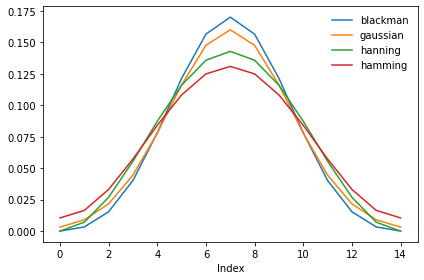
\includegraphics[width=0.8\linewidth]{resources/Images/task3_windows}
        \caption{Созданные окна.}
        \label{fig:task3_windows}
    \end{figure}

    \begin{figure}[H]
        \centering
        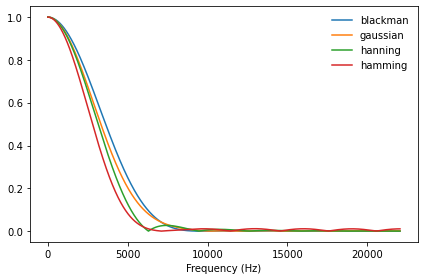
\includegraphics[width=0.8\linewidth]{resources/Images/task3_windows_dft}
        \caption{ДПФ окон.}
        \label{fig:task3_windows_dft}
    \end{figure}

    Из Рис.\ref{fig:task3_windows_dft} видно, что ПДФ окна Хэмминга падает быстрее всех, Блэкмана - медленнее всех,
    а у ПДФ окна Ханнинга самые заметные <<боковые лепестки>>. Но они все очень похожи

    Теперь посмотрим на те же графики в логарифмическом масштабе по $y$.

    \begin{lstlisting}[caption= Получение ДПФ окон в логарифмичесом масштабе по \texttt{y}., label={lst:task3_windows_dft_log}]
plot_window_dfts(windows, names)
decorate(xlabel='Frequency (Hz)', yscale='log')
    \end{lstlisting}

    \begin{figure}[h]
        \centering
        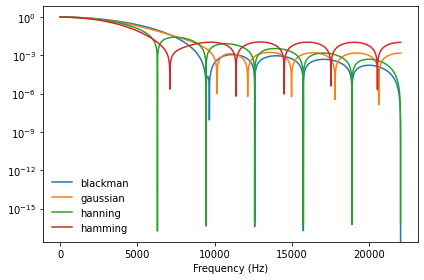
\includegraphics[width=0.8\linewidth]{resources/Images/task3_windows_dft_log}
        \caption{ДПФ окон в логарифмическом масштабе по $y$.}
        \label{fig:task3_windows_dft_log}
    \end{figure}

    Из Рис.\ref{fig:task3_windows_dft_log} видно, что значения окон Хэмминга и Хеннинга падают быстрее остальных.
    Также окна Хэмминга и Гаусса имеют самые стойкие <<боковые лепестки>>. Таким образом можно сделать вывод, что окно
    Ханнинга имеет наилучшее сочетание быстрого падения и минимальных <<боковых лепестков>>.

    В ходе выполнения данного упражнения были изучены различные окна: Хэмминга, Блэкмана, Ханнинга и окно Гаусса.
    Были получены и сравнены их ДПФ в обычном и логарифмическом масштабах. По результатам сравнения был сделан вывод, что
    окно Ханнинга имеет наилучшее сочетание быстрого падения и минимальных <<боковых лепестков>>.

    \newpage

% ---------------------------------------------- Выводы ----------------------------------------------
    \section{Выводы}
    \label{sec:conclusions}

    В ходе выполнения данной лабораторной работы были изучены понятия фильтрации и свёртки, а таже  рассмотрено влияние
    изменения \texttt{std} на преобразование Фурье. Был сделан вывод, при увеличении \texttt{std} гауссово окно сжимается,
    а его БПФ расширяется. Таким образом, между ними существует обратная зависимость. Также были более подробно изучены
    различные окна (Хэмминга, Блэкмана, Ханнинга и Гаусса). Из полученных результатов видно,что окно Ханнинга имеет
    наилучшее сочетание быстрого падения и минимальных <<боковых лепестков>>.

\end{document}